\documentclass[titlepage]{article}
\title{ Computer Workshop Final homework}
\usepackage{url}
\usepackage{graphicx}
\usepackage{hyperref}
\usepackage{geometry}
\geometry{a4paper}
\usepackage{fancyhdr}
\pagestyle{fancy}
\lhead{}
\rhead{CW project}

\author{Hossein Rasipoor \\ 402411458}
\date{1403/11/05}


\begin{document}
\maketitle
\tableofcontents
\newpage

\section{Git and GitHub}
\subsection{Repository Initialization and Commits}
First, I created a repository on my GitHub account. Then, I navigated to the Actions tab and selected the option to create a custom action. I pasted the main.yml file into the editor and committed the changes. After that, I cloned my repository to a local folder on my PC and started writing the content.

\subsection{GitHub Actions for LaTeX Compilation}
In this part, I created a file that compiles LaTeX to PDF with some prompts. To compile the LaTeX file, we need to create a tag using the git tag command, which allows the document to be published as a PDF on GitHub.

\section{Exploration Tasks}
\subsection{Vim Advanced Features}
\begin{itemize}
    \item \textbf{Macros for Automating Repeated Tasks}
\newline
Vim allows users to record and replay a series of keystrokes, known as macros, to automate repetitive tasks. for this we use q for record and @ for register them
    \item \textbf{Search and Replace with Ranges and Patterns}
\newline
Vim's :substitute command allows for complex search-and-replace operations using regular expressions and ranges. pattern:
\newline
:[range]s/pattern/replacement/[flags]

    \item \textbf{Splits and Tabs for Efficient Window Management}
    \newline Splits and tabs in Vim help you manage multiple files or sections simultaneously. Use :split for horizontal splits and :vsplit for vertical ones. Navigate between splits with Ctrl-w + h/j/k/l. For tabs, :tabnew [filename] opens a new tab, and gt/gT switches between them.
\end{itemize}



\subsection{Memory profiling}
\subsubsection{Memory Leak}
memory leak occurs when a program allocates memory but fails to release it, leading to wasted memory and performance issues. This usually happens when references to the memory are lost or it's not properly freed.

\subsubsection{Memory profilers}
Valgrind is an instrumentation framework for building dynamic analysis tools. There are Valgrind tools that can automatically detect many memory management and threading bugs, and profile your programs in detail. You can also use Valgrind to build new tools.

\subsection{GNU/Linux Bash Scripting}

\subsubsection{fzf}
\begin{itemize}
    \item What is fuzzy searching? Give a short description.
    \newline Fuzzy searching is a technique used to find matches that are approximately close to a given search term, even if the term is misspelled or incomplete. It allows for slight variations in spelling, typos, or other errors while still returning relevant results. This approach is useful in situations where exact matches are not necessary, such as when dealing with user input errors or partial information.
    \item Install fzf on your machine and give a description of what the following command does:\\
        \texttt{ls | fzf}
        \newline
        When you run \texttt{ls | fzf}, it lists all files and directories in the current directory and then allows you to interactively search and select one of them using fuzzy matching. As you type, fzf filters and shows the closest matches, making it easier to select files quickly
\end{itemize}

\subsubsection{Using fzf to find your favorite PDF}

\begin{enumerate}
    \item \texttt{"fd -e PDF"}
This command will search for all files with the .PDF extension in the current directory and its subdirectories. The -e option is used to specify the file extension filter
    \item \texttt{"fd -e PDF | fzf"} we use this command for search from list of pdf's that we have
\end{enumerate}

\subsubsection{Opening the file using Zathura}
\texttt{"zathura \$(fd -e PDF | fzf)"} This command will open the PDF you select using Zathura

\section{Git and FOSS}
\subsection{README.md}
i created the README file in github

\subsection{Issues}
created with this title: \textbf{new sample issue for final cw project part 3.2}
\begin{figure}[h]
    \centering
    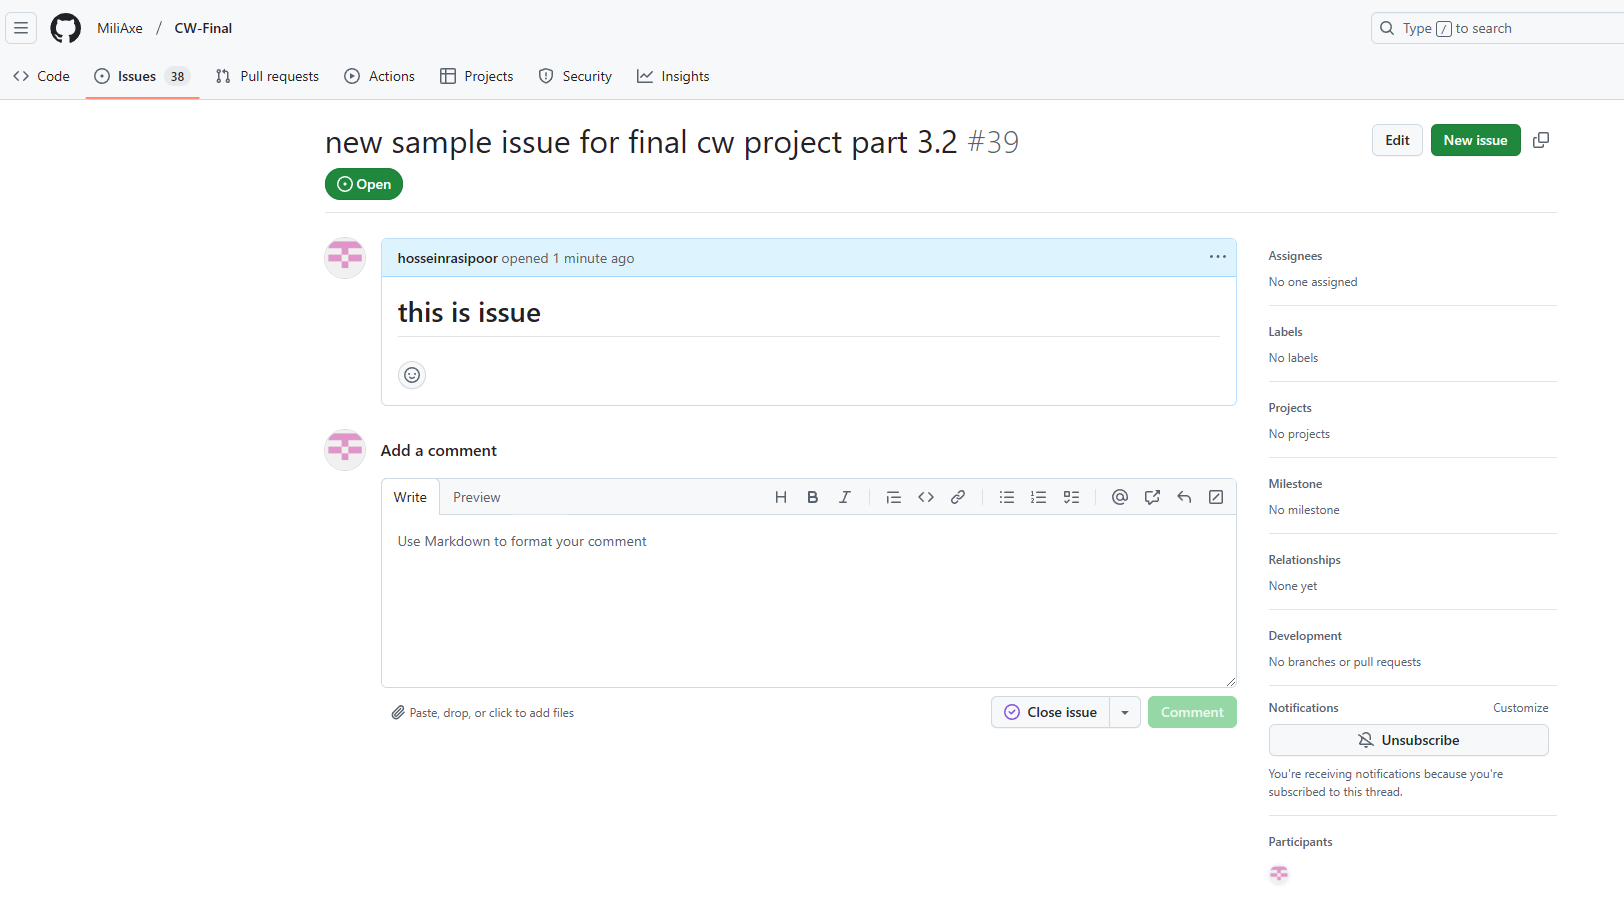
\includegraphics[width=0.55\textwidth]{screenshot.png}
    \caption{issue photo}
\end{figure}

\subsection{FOSS contribution}
Yes, I am interested in contributing to FOSS projects in the future. I am particularly drawn to areas where I can combine my passion for coding with meaningful contributions. For example, I would love to work on improving project documentation, creating tutorials for beginners, or helping with bug fixes and feature implementations. Additionally, I have an interest in enhancing user interfaces and user experiences, so I would be excited to contribute to FOSS projects that focus on design improvements. In general, I think FOSS is a great way to collaborate, learn, and give back to the community, and I am eager to get involved.
\section*{Sources}
\begin{itemize}
    \item this is my refrense for main.yml for action part \url{https://github.com/MiliAxe/CW-Final}
    \item \url{https://www.vim.org/docs.php}
    \item \url{https://valgrind.org/}
    \item and other websites
\end{itemize}

\end{document}
